\title{Assignment 1: CS 215}
\author{Akash Trehan-150050031, Bhavya Bahl-150050110}

\documentclass[11pt]{article}

\usepackage{amsmath}
\usepackage{amssymb}
\usepackage{hyperref}
\usepackage{ulem}
\usepackage{graphicx}
\usepackage[margin=0.5in]{geometry}
\delimitershortfall-1sp
\newcommand\abs[1]{\left|#1\right|}
\begin{document}
\maketitle
$$\mu = Mean,\ \nu=Median,\ \sigma=Standard\ Deviation$$
Ans 1.\begin{center}
$$|\mu-\nu|=\abs{\frac{\sum\limits_{i=1}^nx_i}{n}-\nu}$$
$$= \abs{\frac{\sum\limits_{i=1}^nx_i-n\nu}{n}}$$
$$= \abs{\frac{\sum\limits_{i=1}^n(x_i-\nu)}{n}}$$
$$\le \frac{\sum\limits_{i=1}^n\abs{x_i-\nu}}{n}\ (Extended\ Triangle\ Inequality)$$
$$\le  \frac{\sum\limits_{i=1}^n\abs{x_i-\mu}}{n}\ (\because Absolute\ deviation\ is\ minimum\ for\ median)$$
$$\le \sqrt{\frac{\sum\limits_{i=1}^n(x_i-\mu)^2}{n}}\ (R.M.S \ge A.M)$$
$$\le \sqrt{\frac{\sum\limits_{i=1}^n(x_i-\mu)^2}{n-1}} = \sigma$$

$$Thus\ \abs{\mu-\nu} \le \sigma$$
Hence proved.
\end{center}


\pagebreak
Ans 2.\begin{center}
$$z_i = ax_i + b, a\neq 0$$
$$w_i = cy_i + d, c\neq 0$$

$$So\ \mu_z = a\mu_x + b \ and \ \mu_w = c\mu_y+d$$
$$r(z,w) = \frac{\sum\limits_{i=1}^n(z_i - \mu_z)(w_i - \mu_w)}{\sqrt{{\sum\limits_{i=1}^n(z_i - \mu_z)^2}{\sum\limits_{i=1}^n(w_i - \mu_w)^2}}}$$
$$Now \ z_i - \mu_z = ax_i + b - (a\mu_x +b) = a(x_i - \mu_x) \ \forall i,\ 1\le i \le n$$
$$Similarly \ w_i - \mu_w = c(y_i - \mu_y) \ \forall i,\ 1\le i \le n$$

$$Substituting\ values\ for\ (z_i - \mu_z)\ and\ (w_i - \mu_w), we\ have$$
$$r(z,w) = \frac{\sum\limits_{i=1}^n(a(x_i - \mu_x))(c(y_i - \mu_y))}{\sqrt{{\sum\limits_{i=1}^n(a(x_i - \mu_x))^2}{\sum\limits_{i=1}^n(c(y_i - \mu_y))^2}}}$$
$$= \frac{ac}{|ac|}\frac{\sum\limits_{i=1}^n(x_i - \mu_x)(y_i - \mu_y)}{\sqrt{{\sum\limits_{i=1}^n(x_i - \mu_x)^2}{\sum\limits_{i=1}^n(y_i - \mu_y)^2}}}$$
$$=\frac{ac}{|ac|} r(x,y)= \pm r(x,y) \ (Since\ a\ne0\ and\ c\ne0)$$
\centerline{Hence proved.}\newline
Now, $\frac{ac}{|ac|}=1$ when a and c have the same sign and $\frac{ac}{|ac|}=-1$ when a and c have opposite signs.\newline
Thus r(z,w)=r(x,y) when a and c have same sign and r(z,w)=-r(x,y) when a and c have opposite signs.
\newline
\newline
\end{center}



Ans 3.\begin{center}
$$To\ prove:\ |x_i - \mu| \le \sigma\sqrt{n-1}\ \forall i$$ \newline
By definition of standard deviation
$$\sigma = \sqrt{\frac{\sum\limits_{i=1}^n(x_i-\mu)^2}{n-1}}$$
$$\Rightarrow\ \sigma^2=\frac{\sum\limits_{i=1}^n(x_i-\mu)^2}{n-1}$$
$$\Rightarrow\ \sigma^2\ge\frac{(x_i-\mu)^2}{n-1}, \forall i,1\le i\le n\ (\because\ all\ terms\ are\ positive)$$
$$\Rightarrow\ (n-1)\sigma^2 \ge (x_i-\mu)^2\ (\because\ n-1 > 0)$$
Both sides are positive, so taking square root on both sides we have,
$$\sigma\sqrt{n-1} \ge |x_i-\mu|$$
Hence proved.

\vspace{50px}

\textbf{Instructions for running code}
\begin{enumerate}
\item For Ques 4
\begin{itemize}
\item For first part of the question with random values added between 5 and 10 run file task4\_1.m in MATLAB.
\item For first part of the question with random values added between 100 and 120 run file task4\_2.m in MATLAB.
\end{itemize}
\item For Ques 5
\begin{itemize}
\item Yo
\end{itemize}
\end{enumerate}
\end{center}

Ans 4.\begin{center}
Moving \textbf{Median} filtering produced better relative mean squared error than Moving \textbf{Mean} filtering. The reason is that \textbf{Median is robust to outliers}. This means that the points far away from the mean do not have much effect on the median. This is because the middle element of the set either remains the same or changes to an element closeby. Mean on the other hand depends on the sum of all elements and outliers can have a huge effect on this sum. The following graphs show a really good demonstration of this.
\begin{figure}
  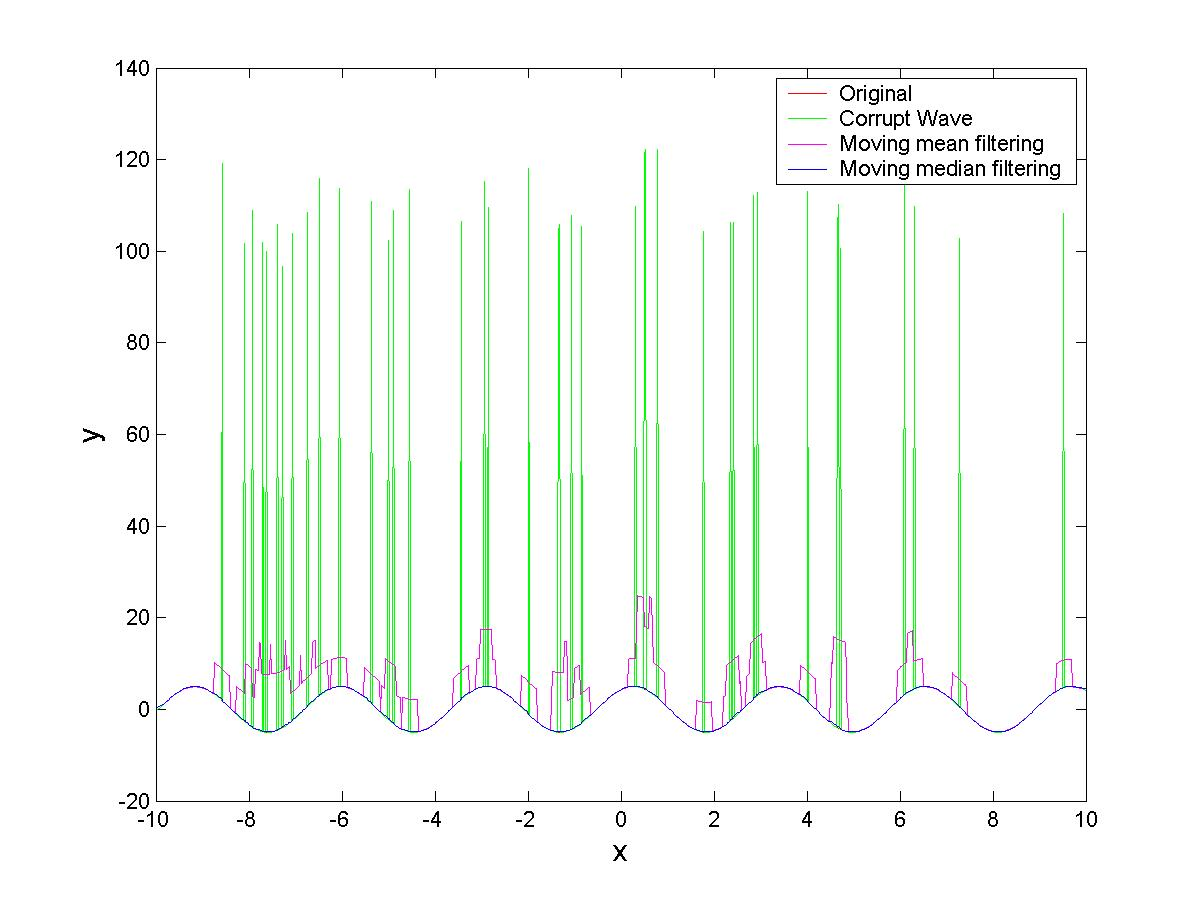
\includegraphics[width=\linewidth]{1.jpg}
  \caption{Task 4(1)}
  \label{fig:task4_1}
\end{figure}
\end{center}
\end{document}